\section{Control Sequences} \label{sec:sequences}
\subsection{Instruction Decoding}
By setting the control signals as described in Section \ref{sec:architecture} appropriately, modules can work together to perform each of the BF instructions. Table \ref{tab:microcode} shows the control sequences that are executed for each BF instruction. The Control Unit implements this as a lookup-table in 3 ROM chips, where the instruction (4 bits), flags (5 bits) and cycle counter (3 bits) act as an address into this table (Figure \ref{fig:decoder}). Given that the CU has to be able to supply a total of 24 different control signals, three 8-bit EEPROM chips have been used to store the microcode lookup-table. More details on the implementation can be found in Section \ref{sec:implementation:cu}. Below we will go through each of the control-sequences listed in Table \ref{tab:microcode}.

\begin{figure}[H]
  \centering
  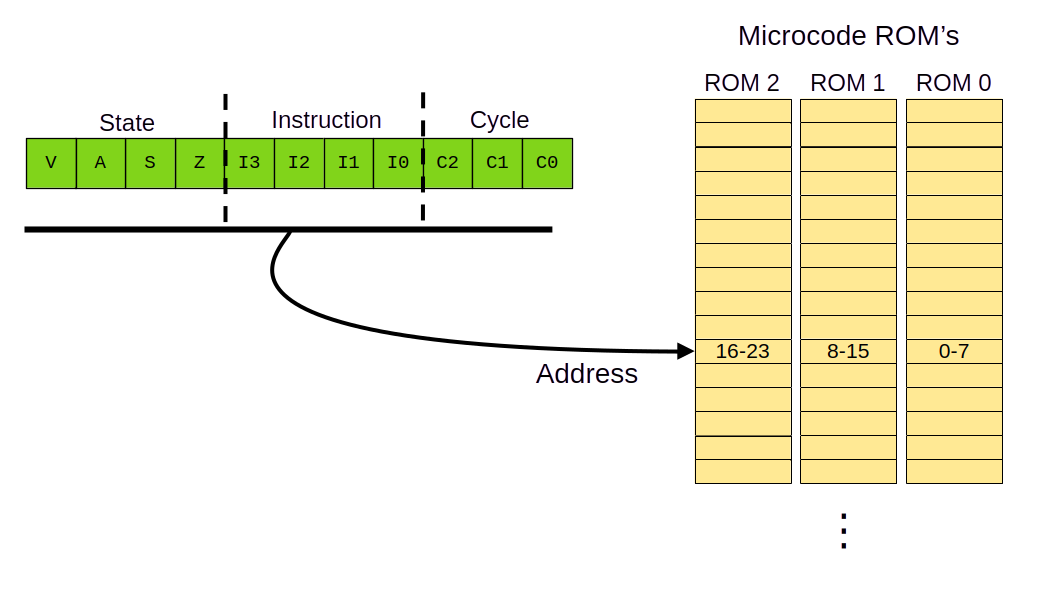
\includegraphics[width=0.9\textwidth]{img/instruction_decoding}
  \caption{Decoding an instruction: the current instruction, flags and cycle-count are used as an index to the three ROM chips that output the control signals corresponding to the current state of the system.}
  \label{fig:decoder}
\end{figure}

\paragraph{No simultaneous INC/DEC signals.} It is important to note that, because of the choice of driving all of the (counting) registers with a common interface (Section \ref{sec:architecture:registerdriver}), only one register can be driven during each clock cycle. That is, the INC and DEC signals can be applied to only one register at a time. 


\subsection{Cycle 0: Instruction Fetch}
The first cycle of each instruction is identical\footnote{The OUT instruction is slightly different but this can be ignored for now. For more information, refer to \label{sec:??}}: A, V, S and Z are loaded into the FB registerand the current instruction (pointed to by IP) is loaded from program ROM into the instruction register. This provides the CU with all the necessary information to determine the control signals for cycle 1: LD\_FB, LD\_I.

\subsection{Modifying Data: \texttt{+} and \texttt{-}} \label{sec:sequences:+-}
\paragraph{PLUS-instruction} The sequence of instructions necessary to execute a \texttt{+} command depends on the state of the system. Three different scenario's have to be taken into account:
\begin{enumerate}
\item (A = 0, S = 0): If the A flag (address-change-flag) is not set, the value in D already corresponds to the value currently pointed to by the DP and no synchronization has to be performed. In that case, its INC signal is immediately asserted to the D register in order for it to increment on the next clock pulse. Referring to Table \ref{tab:registers}, we see only RS0 has to be asserted in conjunction with the INC signal to increment D (register address 0b001). The V-flag must also be set in order to indicate that the value in D has been changed: this is done by asserting the SET\_V signal to FA and latching in the value using the LD(FA) signal: INC, RS0, SET\_V, LD\_FA. Now that the value has been incremented and the corresponding flag has been set, the IP is incremented using the register-driver. The cycle reset signal is asserted at the same time to make sure the next instruction will be loaded on cycle 0: INC, RS2, CR.
\item (A = 1, S = 0): However, when the A flag \emph{was} set, this means that the address has recently changed and the value inside D does not correspond to the value pointed to by the DP in RAM. We therefore need to fetch the current value from RAM by enabling the DP register, enabling the RAM to output its content on the databus and loading the resulting value into D: EN(DP), OE\_RAM, LD(D). From hereon, the next set of control signals is identical to that described above in the case where A was not set.
  \item (S = 1): None of the actions above need to be performed when the S flag is set, which means that we're in the process of skipping a loop-block. In this case, we ignore the command and increment the IP immediately and reset the cycle counter: INC, RS2, CR.
\end{enumerate}


\paragraph{MINUS-instruction} The control signals necessary to perform the \texttt{-} command are similar to those of the \texttt{+} command, the only difference being the DEC signal to perform a subtraction rather than addition.


\begin{figure}[H]
  \centering
  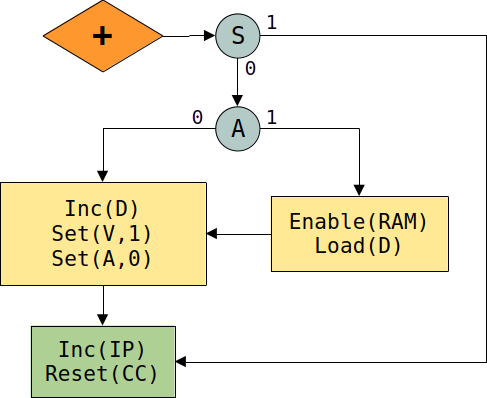
\includegraphics[scale=0.3]{img/plusalg}
  \caption{Block diagram for the \texttt{+} command. The diagram for the \texttt{-} command is equivalent (using \texttt{Dec} rather than \texttt{Inc}).}
  \label{fig:plusalg}
\end{figure}

\subsection{Moving the Pointer: \texttt{<} and \texttt{>}} \label{sec:sequences:<>}
\paragraph{RIGHT-instruction} Moving the datapointer one cell to the right requires similar instructions compared to PLUS instruction, the difference being that we increment the DP-register rather than the D-register. Similarly, we consider three different scenario's, branching on the V-flag instead of the A-flag:
%
\begin{enumerate}
\item (V = 0, S = 0): If the V-flag is not set, it means that the value we point to hasn't changed and we don't need to care about synchronization. The DP (register address 010) is incremented immediately and the A-flag is set to indicate we changed the address and are now out of sync: INC, RS1, SET\_A, LD\_FA. In the following cycle, we move to the next instruction: INC, RS2, CR.
\item (V = 1, S = 0): In the case that V \emph{was} set during one of the previous instructions, we need to write the updated value (present in the D-register) back to RAM before moving the pointer. This is achieved by enabling the value in D onto the databus and setting the RAM module to write-mode. Furthermore, the V-flag needs to be cleared. This is achieved by loading FA without setting any signals; this will effectively reset both A and V back to zero: EN\_D, WE\_RAM, LD\_FA. Now that the RAM contains the updated value, it is safe to move the DP to the next cell. The control sequence to do this is identical to the sequence described in the (V = 0)-scenario.
\item (S = 1): None of the actions above need to be performed when the S flag is set, which means that we're in the process of skipping a loop-block. In this case, we ignore the command and increment the IP immediately and reset the cycle counter: INC, RS2, CR.
\end{enumerate}

\paragraph{LEFT-instruction} The control signals necessary to perform the \texttt{<} command are similar to those of the \texttt{>} command, the only difference being the DEC signal to perform a subtraction rather than addition.


\begin{figure}[H]
  \centering
  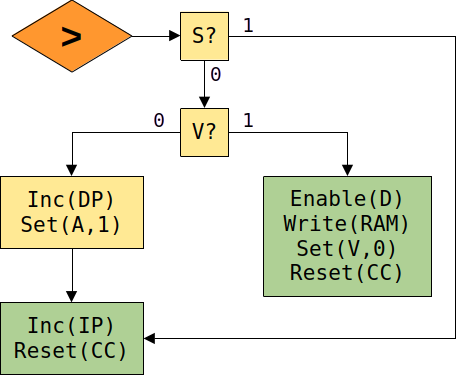
\includegraphics[scale=0.3]{img/rightalg}
  \caption{Block diagram for the \texttt{>} command. The diagram for the \texttt{<} command is equivalent (using \texttt{Dec} rather than \texttt{Inc}).}
  \label{fig:rightalg}
\end{figure}

\subsection{Conditional Jumping: \texttt{[} and \texttt{]}}
These are by far the most complicated instructions that require a lot of additional logic. Because the BF instruction set lacks a JMP-instruction where some argument holds the destination address, the computer has to store the address of the opening \texttt{[}-command in case it needs to loop back when the time comes. When a loop is skipped, the LS (Loop Skip) register is used to determine when execution should resume. This leads to multiple scenario's depending on the state of A, Z and S.
  
  \paragraph{LOOP\_START-instruction} 
  
  \begin{enumerate}
  \item (A = 0, Z = 1, S = 0): In the first scenario, where A is not set (the D-register is up-to-date) and the Z-flag is set, we can immediately conclude that this loop should be skipped over. Hence, the LS-register is incremented and the next instruction is loaded (to be ignored until the LS-register becomes 0 again). Since LS is addressed by the register driver at address 101, this is done using the control sequence INC, RS0, RS2. In the next cycle, the IP is incremented and the cycle-counter is reset to move to the next instruction: INC, RS2, CR.

  \item (A = 0, Z = 0, S = 0): In the second scenario, the A-flag is still not set but the Z-flag for the D-register is not set either, meaning that control \emph{should} enter the loop. It takes 3 cycles to do so: increment the stack-pointer (cycle 1), write the current IP to this address on the stack (cycle 2) and move to the next instruction (cycle 3). The corresponding control sequences are therefore:
    \begin{enumerate}
    \item INC, RS0, RS1
    \item WE\_RAM, EN\_SP, EN\_IP
    \item INC, RS2, CR
    \end{enumerate}

  \item (A = 1, S = 0): In the third scenario the A-flag \emph{is} set, which means that we should first load the current value from RAM into the D-register (cycle 1) and reset the flag: OE\_RAM, LD\_D, LD\_FA, CR. The cycle count is immediately reset to 0 without incrementing the instruction pointer. This means the same instruction is reloaded with updated flags on the next iteration, putting the system into either one of the states above (either scenario 1 or 2, depending on the value of Z).

  \item (S = 1): In the final scenario, we are in the process of skipping code, indicated by the S-flag (S = 1). In this case, we have encountered a nested loop that needs to be skipped over, so we increment the LS-register once more to account for another pair of nested \texttt{[]}'s (cycle 1) and then continue to the next instruction (cycle 2).
    \begin{enumerate}
    \item INC, RS0, RS2
    \item INC, RS2, CR
    \end{enumerate}
    Note that these instructions could not take place in the same cycle due to the usage of the register driver, which can only increment one register per cycle.
  \end{enumerate}


  \paragraph{LOOP\_END-instruction}
  \begin{enumerate}
  \item (A = 0, Z = 1, S = 0): In the first scenario, which takes 2 cycles to execute, there is a known (synchronized) zero in the D-register (A = 0). This means we can immediately choose to exit the loop. To do so, the stack-pointer is decremented (cycle 1) to point at the previous value on the stack. In cycle 2, the IP is incremented as usual:
    \begin{enumerate}
    \item DEC, RS0, RS1  
    \item INC, RS2, CR
    \end{enumerate}

  \item (A = 0, Z = 0, S = 0): In the second scenario, there is a known nonzero value in D, this means we must loop back to the IP stored on the top of the stack. This value is loaded into the IP-register by enabling the SP and RAM and setting the LD signal for the IP-register (cycle 1). On the second cycle, this new IP (pointing to a \texttt{[}) is incremented to re-enter the loop.
      \begin{enumerate}
      \item EN\_SP, OE\_RAM, LD\_IP
      \item INC, RS2, CR
      \end{enumerate}
      
    \item (A = 1, S = 0): In the third scenario, the contents of D are not yet synchronized with the RAM, so we first need to load it in. After loading the value into D, the flags and cycle counter are reset to put the system back into one of the previously defined states: OE\_RAM, LD\_D, LD\_FA, CR.

    \item (S = 1): Finally, when already in the process of skipping a loop, the LS-register is decremented before moving to the next instruction before resetting the cycle counter and incrementing the IP:
      \begin{enumerate}
      \item DEC, RS0, RS2
      \item INC, RS2, CR
      \end{enumerate}
  \end{enumerate}

\begin{figure}[H]
  \centering
  \mbox{}\hfill
  \begin{subfigure}[t]{0.4\linewidth}
    \centering
    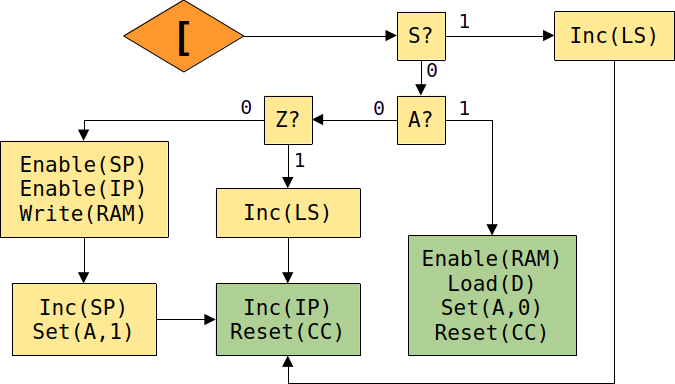
\includegraphics[scale=0.3]{img/loopstartalg}
    \caption{Block diagram for the loop-start command.}
    \label{fig:loopstartalg}
  \end{subfigure}
  \hfill
  \begin{subfigure}[t]{0.4\linewidth}
    \centering
    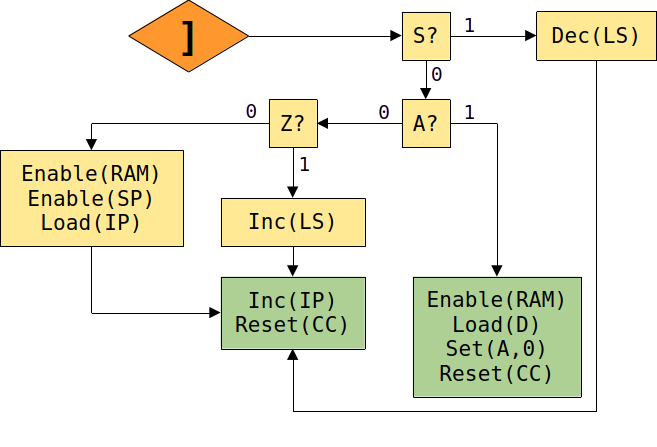
\includegraphics[scale=0.3]{img/loopendalg}
    \caption{Block diagram for the loop-end command.}
    \label{fig:loopendalg}
  \end{subfigure}
  \hfill\mbox{}

  \caption{}
  \label{fig:loopalg}
\end{figure}


\subsection{Output: \texttt{.}} \label{sec:sequences:output}

\paragraph{Handshake:} Due to the asynchronous nature of the output peripheral, it is necessary to enter into a handshake protocol whenever a byte is put on the bus for display. In this protocol, the K flag is used to communicate between the CPU and the IO module: it is set by the IO module to indicate that it has read the data from the bus, and reset by the CU to indicate that the handshake has been received and completed:

\begin{enumerate}
\item The CU asserts the EN\_OUT signal and enables the module that contains the current value (either D when A = 0 or RAM when A = 1), such that its contents appear on the databus:\\EN\_OUT, (EN\_D or OE\_RAM).
\item The output module is notified of this through the EN\_OUT signal and reads this value from the bus. When done, it sets the K-flag.
\item After enabling the data on the bus, the CU repeatedly checks the K-flag. When it becomes 1, the CU knows that the data has been successfully taken from the bus, at which point the supplying module (D or RAM) can disable its outputs. The CU then finalizes the handshake by resetting the K-flag. As soon as the output module notices that the K-flag was reset, it starts waiting for its next instruction.
  \begin{enumerate}
  \item K = 0: CR, (EN\_D or OE\_RAM)
  \item K = 1: CLR\_K, INC, RS2, CR   
  \end{enumerate}
\end{enumerate}


\paragraph{Cycle 0:} As mentioned briefly before, the OUT instruction is the only instruction that has a slightly different cycle 0 control sequence associated with it. This is because the waiting-loop is implemented by simply resetting the cycle count, such that the instruction is loaded in again but may now branch differently depending on the value of K, which might change in the meantime. However, the data on the bus should remain valid for the entire duration of the loop, since the output module may read from it asynchronously. To accommodate for this, the 0-cycle for the OUT instruction enables either D or RAM, depending on the value of the A-flag. This does no harm whenever the sequence is encountered outside of the loop, but does keep the data valid during one. Cycle 0 for the OUT opcode therefore consists of these control signals: LD\_FB, LD\_I, (EN\_D or EN\_RAM).

\subsection{Input: \texttt{,}} \label{sec:sequences:input}
\paragraph{Handshake:} Similar to the output command, the input command implements a handshake protocol to make sure that the databus is claimed by the input-device for the exact right amount of time, in order for the system to reliably read its contents. This happens using the same K-flag that was used in the output handshake.
\begin{enumerate}
\item The CU asserts the EN\_IN signal to let the input-device know that it can claim ownership of the bus.
\item The input-devices receives the EN\_IN signal and puts a value onto the bus (see below for the difference between immediate and buffered input-mode). When the data is ready, it sets the K-flag.
\item After asserting the EN\_IN signal, the CU waits for the K-flag by continuously resetting the cycle counter and branching on the value of K. Once that becomes high, it loads the data into the D register and sets the V-flag:
  \begin{itemize}
  \item K = 0: CR
  \item K = 1: LD\_D, SET\_V, LD\_FA
  \end{itemize}
\item To finalize the handshake, the K-flag is cleared by the CU by setting the CLR\_K signal.  
\end{enumerate}

\paragraph{Input-Modes:} The input peripheral (probably) manages an internal buffer to serve subsequent bytes from to the system, which might be empty when the request for input arrives. When this happens, it is up to the peripheral to decide upon one of 2 options:
\begin{enumerate}
\item Wait for the buffer to contain data. Only then set the K-flag (buffered mode).
\item Assert zero's to the bus and set the K-flag immediately (immediate mode).
\end{enumerate}
In our implementation of the IO-module (see \ref{sec:implementation:io}), both modes are supported and can be selected from in the options menu.

\begin{figure}[H]
  \centering
  \mbox{}\hfill
  \begin{subfigure}[t]{0.4\linewidth}
    \centering
    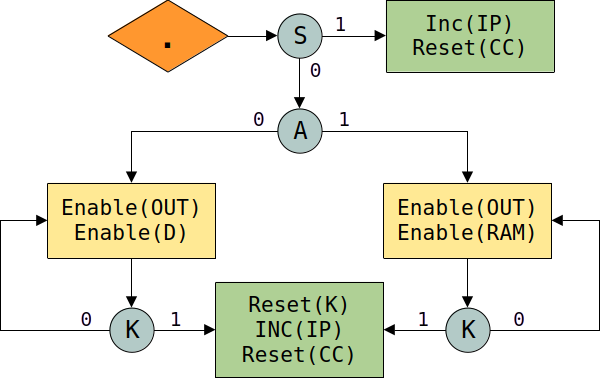
\includegraphics[scale=0.3]{img/outputalg}
    \caption{Block diagram for the output command.}
    \label{fig:inputbufalg}
  \end{subfigure}
  \hfill
  \begin{subfigure}[t]{0.4\linewidth}
    \centering
    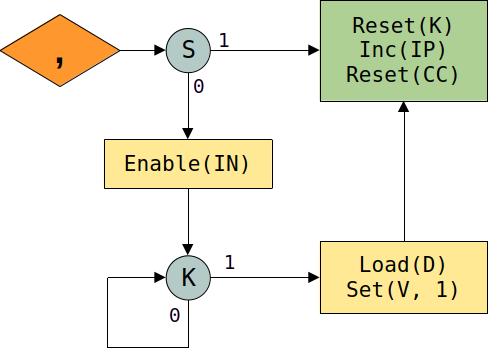
\includegraphics[scale=0.3]{img/inputalg}
    \caption{Block diagram for the input command.}
    \label{fig:inputimalg}
  \end{subfigure}
  \hfill\mbox{}
  \caption{}
  \label{fig:inputalg}
\end{figure}

\subsection{Non-BF instructions} \label{seq:sequences:nonbf}
Several non-BF instructions have been implemented for debugging purposes and to initialization at startup. Furthermore, the common extension \emph{Random Brainf*ck} \cite{esolangs-rbf} is implemented as an additional instruction (RAND) that acts just like the IN instruction, except now a random number appears on the bus rather than user input (handled by the IO module as well). All non-BF opcodes are listed and described below.

\subsubsection{\texttt{NOP}}
The NOP instruction does nothing. It simply increments the IP and resets the cycle count to move to the next instruction.

\subsubsection{\texttt{WAIT\_EXT}}
The WAIT\_EXT instruction (\emph{wait for external device}) should be the first instruction in the program binary and simply loops on the K-flag, waiting for an external peripheral to set it to 1. When this happens, the CU immediately resets the flag using the CLR\_K signal. Both the BF system and the IO module will now be ready for operation:
\begin{itemize}
 \item (K = 0): CR
 \item (K = 1): CLR\_K, K\_REC, INC, RS2, CR
\end{itemize}

\begin{figure}[H]
  \centering
  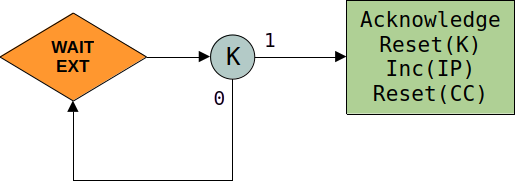
\includegraphics[scale=0.4]{img/waitextalg}
  \caption{Block diagram for the WAIT\_EXT instruction.}
  \label{fig:rightalg}
\end{figure}


\subsubsection{\texttt{INIT}} \label{sec:sequences:init}
In any BF program it is assumed that all memory is zero-initialized. In practice, SRAM-modules will contain random values at startup, so the assembler must add a preamble to the main code (after the initial WAIT\_EXT handshake) in order to initialize the RAM (or at least part of it) to 0. While this can be handled using canonical BF commands, initializing one cell at a time using a sequence of \texttt{[-]} commands, it is much faster to write directly to RAM. This is the purpose of the INIT instruction: for each INIT instruction, a contiguous chunk of 256 memory-cells will be zero-initialized. Since it is guaranteed that the D register contains a zero after reset, this value can directly be written into RAM on the first cycle of INIT while also incrementing the LS and DP registers. DP is incremented to move through the memory-space whereas LS is incremented in order to be able to count to 256, at which point the S flag will go low again due to the LS register overflowing back to 0. If more memory needs to be initialized, the assembler can simply concatenate multiple INIT instructions.
\begin{enumerate}
\item Write a zero to the current cell: EN\_D, WE\_RAM, INC, RS0, RS2
\item Increment the LS-register: LD\_FB, INC, RS1
\item Depending on whether the LS-register wrapped around (256 cells initialized), either move to the next cell or finalize by incrementing the IP and resetting the cycle-counter.
  \begin{itemize}
  \item (S = 0): INC, RS2, CR
  \item (S = 1): CR
  \end{itemize}
\end{enumerate}
After the appropriate number of INIT instructions have been execured, the HOME instruction (see \ref{sec:sequences:home} must be called in order for the DP to return back to the start of the memory (0x0100).

\subsubsection{\texttt{HOME}} \label{sec:sequences:home}
In order for the datapointer to return to its starting position after initialization (and before the main program runs), the \texttt{HOME} instruction is provided. The only thing it does is send the reset signal to the datapointer using the CLR\_DP signal.

\subsubsection{\texttt{HLT}}
The \texttt{HLT} instruction halts the clock and (temporarily) stops the program by asserting the HLT signal. The assembler will place a HLT instruction after initialization (\texttt{INIT}) and after the final instruction of the main program. This former allows the user to manually start the program after the system has been fully set up and the latter prevents the program from continuing into invalid memory after it has executed its final command. Furthermore, the assembler can interpret an exclamation mark (\texttt{!}) as a \texttt{HLT} in the BF-code to set breakpoints for debugging.

When the system is resumed and cycle 2 of the HLT instruction is reached, the IP is incremented as usual in the final cycle of any instruction: INC, RS2, CR.

\subsubsection{\texttt{ERR}}
The \texttt{ERR} instruction enables the ERR signal and halts the clock: ERR, HLT. It therefore acts similarly to a regular \texttt{HLT}, but indicates to the end user that the system was halted due to an error (and it is therefore probably not wise to resume the system anyway). Furthermore, there is no second cycle defined to increment IP and go beyond this point in the program.

Every undefined state in the microcode table implicitly contains the \texttt{ERR} sequence. If for some reason a state occurs that maps to the \texttt{ERR} command, the clock will be halted and some indicator on the Control Unit should light up to let its users know that something has gone terribly wrong and the computer has reached an unreachable state.

\subsection{Microcode table}
Table \ref{tab:microcode} shows each of the control sequences described in previous sections sections. Please note that in order to simplify notation, the control signals RS0, RS1 and RS2 have not been used to indicate register selection. Instead, the module to which the instruction (INC/DEC) is applied is provided in brackets. For example, incrementing the SP register would require control signals INC, RS0, RS1 which is denoted in Table \ref{tab:microcode} as INC(SP).
\newpage
\begin{landscape}
  \begin{longtable}[c] {c|cccc|c|llllll}
                     Instr        & V & A & Z(LS) & Z(D) & Cycle & \multicolumn{6}{c}{Control Signals}                      \\ \hline
    \rowcolor{White} Any          &   &   &       &      & 0     & EN(IP)   & LD(I)    &         &        &        &        \\ \hline
    \rowcolor{Gray}  \texttt{+}   &   & 0 & 1     &      & 1     & CE(D)    & VE(CU)   & LD(F)   &        &        &        \\
    \rowcolor{Gray}               &   & 0 & 1     &      & 2     & CE(IP)   & CR(CU)   &         &        &        &        \\    
    \rowcolor{White}              &   & 1 & 1     &      & 1     & EN(DP)   & LD(D)    & OE(RAM) & LD(F)  & CR(CU) &        \\
    \rowcolor{Gray}               &   &   & 0     &      & 1     & CE(IP)   & CR(CU)   &         &        &        &        \\ \hline
    
    \rowcolor{White} \texttt{-}   &   & 0 & 1     &      & 1     & CE(D)    & DEC(D)   & VE(CU)  & LD(F)  &        &        \\
    \rowcolor{White}              &   & 0 & 1     &      & 2     & CE(IP)   & CR(CU)   &         &        &        &        \\
    \rowcolor{Gray}               &   & 1 & 1     &      & 1     & EN(DP)   & LD(D)    & OE(RAM) & LD(F)  & CR(CU) &        \\
    \rowcolor{White}              &   &   & 0     &      & 1     & CE(IP)   & CR(CU)   &         &        &        &        \\ \hline
    
    \rowcolor{Gray}  \texttt{>}   & 0 &   & 1     &      & 1     & CE(DP)   & AE(CU)   & LD(F)   &        &        &        \\
    \rowcolor{Gray}               & 0 &   & 1     &      & 1     & CE(IP)   & CR(CU)   &         &        &        &        \\
    \rowcolor{White}              & 1 &   & 1     &      & 1     & EN(D)    & EN(DP)   & WE(RAM) & LD(F)  & CR(CU) &        \\
    \rowcolor{Gray}               &   &   & 0     &      & 1     & CE(IP)   & CR(CU)   &         &        &        &        \\ \hline
    
    \rowcolor{White} \texttt{<}   & 0 &   & 1     &      & 1     & CE(DP)   & DEC(DP)  & AE(CU)  & LD(F)  &        &        \\
    \rowcolor{White}              & 0 &   & 1     &      & 2     & CE(IP)   & CR(CU)   &         &        &        &        \\
    \rowcolor{Gray}               & 1 &   & 1     &      & 1     & EN(D)    & EN(DP)   & WE(RAM) & LD(F)  & CR(CU) &        \\
    \rowcolor{White}              &   &   & 0     &      & 1     & CE(IP)   & CR(CU)   &         &        &        &        \\ \hline
    
    \rowcolor{Gray}  \texttt{[}   &   & 0 & 1     & 1    & 1     & CE(LS)   &          &         &        &        &        \\
    \rowcolor{Gray}               &   & 0 & 1     & 1    & 2     & CE(IP)   & CR(CU)   &         &        &        &        \\      
    \rowcolor{White}              &   & 0 & 1     & 0    & 1     & CE(SP)   &          &         &        &        &        \\
    \rowcolor{White}              &   & 0 & 1     & 0    & 2     & WE(RAM)  & EN(SP)   & EN(IP)  &        &        &        \\
    \rowcolor{White}              &   & 0 & 1     & 0    & 3     & CE(IP)   & CR(CU)   &         &        &        &        \\
    \rowcolor{Gray}               &   & 1 & 1     &      & 1     & EN(DP)   & LD(D)    & OE(RAM) &        &        &        \\
    \rowcolor{Gray}               &   & 1 & 1     &      & 2     & LD(F)    & CR(CU)   &         &        &        &        \\
    \rowcolor{White}              &   &   & 0     &      & 1     & CE(LS)   &          &         &        &        &        \\
    \rowcolor{White}              &   &   & 0     &      & 2     & CE(IP)   & CR(CU)   &         &        &        &        \\ \hline
    
    \rowcolor{White} \texttt{]}   &   & 0 & 1     & 1    & 1     & CE(SP)   & DEC(SP)  &         &        &        &        \\
    \rowcolor{White}              &   & 0 & 1     & 1    & 2     & CE(IP)   & CR(CU)   &         &        &        &        \\
        
    \rowcolor{Gray}               &   & 0 & 1     & 0    & 1     & EN(SP)   & EN(RAM)  & LD(IP)  &        &        &        \\
    \rowcolor{Gray}               &   & 0 & 1     & 0    & 2     & CE(IP)   & CR(CU)   &         &        &        &        \\
    \rowcolor{White}              &   & 1 & 1     &      & 1     & EN(DP)   & EN(RAM)  & LD(D)   &        &        &        \\
    \rowcolor{White}              &   & 1 & 1     &      & 2     & LD(F)    & CR(CU)   &         &        &        &        \\
    \rowcolor{Gray}               &   &   & 0     &      & 1     & CE(LS)   & DEC(LS)  &         &        &        &        \\ 
    \rowcolor{Gray}               &   &   & 0     &      & 2     & CE(IP)   & CR(CU)   &         &        &        &        \\ \hline
    
    \rowcolor{Gray}  \texttt{.}   &   & 0 & 1     &      & 1     & PRE(SCR) & EN(D)    & CE(IP)  & CR(CU) &        &        \\
    \rowcolor{White}              &   & 1 & 1     &      & 1     & EN(DP)   & EN(RAM)  & LD(D)   &        &        &        \\
    \rowcolor{White}              &   & 1 & 1     &      & 2     & PRE(SCR) & EN(D)    & CE(IP)  & CR(CU) &        &        \\
    \rowcolor{Gray}               &   &   & 0     &      & 1     & CE(IP)   & CR(CU)   &         &        &        &        \\ \hline
    
    \rowcolor{White} \texttt{,}   & 0 &   & 1     &      & 1     & EN(KB)   & LD(D)    &         &        &        &        \\
    \rowcolor{White}              & 0 &   & 1     &      & 2     & EN(IP)   & LD(I)    &         &        &        &        \\
    \rowcolor{Gray}               & 0 &   & 1     & 0    & 3     & VE(CU)   & LD(F)    & CE(IP)  & CR(CU) &        &        \\
    \rowcolor{White}              & 0 &   & 1     & 1    & 3     & CR(CU)   &          &         &        &        &        \\   
    \rowcolor{Gray}               & 1 &   & 1     &      & 1     & EN(D)    & EN(DP)   & WE(RAM) &        &        &        \\
    \rowcolor{Gray}               & 1 &   & 1     &      & 2     & LD(F)    & CR(CU)   &         &        &        &        \\
    \rowcolor{White}              &   &   & 0     &      & 1     & CE(IP)   & CR(CU)   &         &        &        &        \\ \hline
    
    \rowcolor{Gray}  \texttt{'}   & 0 &   & 1     &      & 1     & EN(KB)   & LD(D)    & VE(CU)  & LD(F)  & CE(IP) & CR(CU) \\
    \rowcolor{White}              & 1 &   & 1     &      & 1     & EN(D)    & EN(DP)   & WE(RAM) &        &        &        \\
    \rowcolor{White}              & 1 &   & 1     &      & 2     & EN(KB)   & LD(D)    & VE(CU)  & LD(F)  & CE(IP) & CR(CU) \\
    \rowcolor{Gray}               &   &   & 0     &      & 1     & CE(IP)   & CR(CU)   &         &        &        &        \\ \hline
    \rowcolor{White} \texttt{NOP} &   &   &       &      & 1     & CE(IP)   & CR(CU)   &         &        &        &        \\ \hline
    \rowcolor{Gray}  \texttt{ERR} &   &   &       &      &       & ERR(CU)  & HLT(CLC) &         &        &        &        \\ \hline

    \caption{Control signals for each of the BF instructions in different scenario's, depending on the state flags. Note that in order to distinguish between the two input modes, the regular comma (\texttt{,}) and the apostrophe (\texttt{'}) are used for buffered and immediate inputs respectively. See also Section \ref{sec:architecture:signals:input}.}
    \label{tab:microcode}
  \end{longtable}
\end{landscape}





